%%%%%%%%%%%%%%%%%%%%%%%%%%%%%%%%%%%%%%%%%%%%%%%%%%%%%%%%%%%%%%%%
%  文章模板:A4 纸,小五字,单列(可根据要求改双列 twocolumn)
%%%%%%%%%%%%%%%%%%%%%%%%%%%%%%%%%%%%%%%%%%%%%%%%%%%%%%%%%%%%%%%%
\documentclass[a4paper,11pt,onecolumn,twoside]{article}

%%%%%%%%%%%%%%%%%%%%%%%%%%%%%%%%%%%%%%%%%%%%%%%%%%%%%%%%%%%%%%%%
%  packages
%    这部分声明需要用到的包
%%%%%%%%%%%%%%%%%%%%%%%%%%%%%%%%%%%%%%%%%%%%%%%%%%%%%%%%%%%%%%%%
\usepackage{CTEX}
\usepackage{fancyhdr}
\usepackage{amsmath,amsfonts,amssymb,graphicx}    % EPS 图片支持
\usepackage{subfigure}   % 使用子图形
\usepackage{indentfirst} % 中文段落首行缩进
\usepackage{bm}          % 公式中的粗体字符(用命令\boldsymbol)
\usepackage{multicol}    % 正文双栏
\usepackage{indentfirst} % 中文首段缩进
\usepackage{picins}      % 图片嵌入段落宏包 比如照片
\usepackage{abstract}    % 2栏文档,一栏摘要及关键字宏包
\usepackage{float}
\usepackage{titlesec}
\usepackage[labelsep=quad,belowskip=-5pt,aboveskip=5pt,font=small]{caption}
\usepackage{array}
\usepackage[boxruled]{algorithm2e}
\usepackage{algorithmicx}   %伪代码
\usepackage{algpseudocode}  %伪代码
\usepackage{bm}         % 公式符号加粗
\usepackage{enumerate}

% \usepackage[superscript,biblabel]{cite} 
% \usepackage[super,square]{natbib}

%%%%%%%%%%%%%%%%%%%%%%%%%%%%%%%%%%%%%%%%%%%%%%%%%%%%%%%%%%%%%%%%
%  lengths
%    下面的命令重定义页面边距,使其符合中文刊物习惯。
%%%%%%%%%%%%%%%%%%%%%%%%%%%%%%%%%%%%%%%%%%%%%%%%%%%%%%%%%%%%%%%%
\addtolength{\topmargin}{-54pt}
\setlength{\oddsidemargin}{-0.9cm}  % 3.17cm - 1 inch
\setlength{\evensidemargin}{\oddsidemargin}
\setlength{\textwidth}{17.00cm}
\setlength{\textheight}{24.00cm}    % 24.62

\setmainfont{Times New Roman}
\setsansfont{Times New Roman}
\setmonofont{Consolas}
\setlength{\columnsep}{8mm}

\titlespacing*{\section}
{0pt}{2ex}{3.5ex}


%%%%%%%%%%%%%%%%%%%%%%%%%%%%%%%%%%%%%%%%%%%%%%%%%%%%%%%%%%%%%%%%
%  定义标题格式,包括title,author,affiliation,email等。
%  在任何用到中文的地方,用\begin{CJK} ... \end{CJK}将其括起来。
%%%%%%%%%%%%%%%%%%%%%%%%%%%%%%%%%%%%%%%%%%%%%%%%%%%%%%%%%%%%%%%%

% \renewcommand{\baselinestretch}{1.1} %定义行间距

\setlength{\baselineskip}{16pt}
\parindent 22pt %重新定义缩进长度

%%%%%%%%%%%%%%%%%%%%%%%%%%%%%%%%%%%%%%%%%%%%%%%%%%%%%%%%%%%%%%%%
% 标题,作者,通信地址定义
%%%%%%%%%%%%%%%%%%%%%%%%%%%%%%%%%%%%%%%%%%%%%%%%%%%%%%%%%%%%%%%%

\title{\huge{\textbf{基于超像素表达的面向目标提取最优分割算法}}}
\author{王金旺\\[2pt]
\normalsize
武汉大学电子信息学院,湖北,武汉,430079 \\[2pt]}
\date{}  % 这一行用来去掉默认的日期显示

%%%%%%%%%%%%%%%%%%%%%%%%%%%%%%%%%%%%%%%%%%%%%%%%%%%%%%%%%%%%%%%%
% 首页页眉页脚定义
%%%%%%%%%%%%%%%%%%%%%%%%%%%%%%%%%%%%%%%%%%%%%%%%%%%%%%%%%%%%%%%%
\fancypagestyle{plain}
{
\fancyhf{}
\lhead{第~XX~卷\quad 第~X~期\\
{2017~年~06~月}}
\chead{\centering{武汉大学学报$\boldsymbol{\cdot}$信息科学版}\\
{Geomatics and Information Science of Wuhan University}}
\rhead{{Vol. XX, No. XX}\\
{June. 2017}}
\lfoot{}
\cfoot{}
\rfoot{}
}

%%%%%%%%%%%%%%%%%%%%%%%%%%%%%%%%%%%%%%%%%%%%%%%%%%%%%%%%%%%%%%%%
% 首页后根据奇偶页不同设置页眉页脚
% R,C,L分别代表左中右,O,E代表奇偶页
%%%%%%%%%%%%%%%%%%%%%%%%%%%%%%%%%%%%%%%%%%%%%%%%%%%%%%%%%%%%%%%%
\pagestyle{fancy}
\fancyhf{}
\fancyhead[RE]{2017年6月}
\fancyhead[CE]{武汉大学学报$\cdot$信息科学版}
\fancyhead[LE,RO]{\thepage}
\fancyhead[CO]{王金旺:基于超像素表达的面向目标提取最优分割算法}
\fancyhead[LO]{第~XX~卷~第~X~期}
\lfoot{}
\cfoot{}
\rfoot{}


%%%%%%%%%%%%%%%%%%%%%%%%%%%%%%%%%%%%%%%%%%%%%%%%%%%%%%%%%%%%%%%%
% 正文两栏环境不允许float环境,比如 figure, table。所以重新定义
% figure,使之可以浮动到你想要的位置。table也同样,把figure改为
% table就可以。
%%%%%%%%%%%%%%%%%%%%%%%%%%%%%%%%%%%%%%%%%%%%%%%%%%%%%%%%%%%%%%%%
\newenvironment{figurehere}
  {\def\@captype{figure}}
  {}
\makeatother

\renewcommand\figurename{图}

\renewcommand\refname{\zihao{5}\centerline{参~考~文~献}}

\begin{document}

%%%%%%%%%%%%%%%%%%%%%%%%%%%%%%%%%%%%%%%%%%%%%%%%%%%%%%%%%%%%%%%%
%  自定义命令
%%%%%%%%%%%%%%%%%%%%%%%%%%%%%%%%%%%%%%%%%%%%%%%%%%%%%%%%%%%%%%%%
% 此行使文献引用以上标形式显示
\newcommand{\supercite}[1]{\textsuperscript{\cite{#1}}}

%%%%%%%%%%%%%%%%%%%%%%%%%%%%%%%%%%%%%%%%%%%%%%%%%%%%%%%%%%%%%%%%
%  显示title,并设页码为空(按杂志社要求)
%%%%%%%%%%%%%%%%%%%%%%%%%%%%%%%%%%%%%%%%%%%%%%%%%%%%%%%%%%%%%%%%
\maketitle

%%%%%%%%%%%%%%%%%%%%%%%%%%%%%%%%%%%%%%%%%%%%%%%%%%%%%%%%%%%%%%%%
%%%%%%%%%%%%%%%%%%%%%%%%%%%%%%%%%%%%%%%%%%%%%%%%%%%%%%%%%%%%%%%%
%  中文摘要
%  调整摘要、关键词,中图分类号的页边距
%  中英文同时调整
%%%%%%%%%%%%%%%%%%%%%%%%%%%%%%%%%%%%%%%%%%%%%%%%%%%%%%%%%%%%%%%%

% \setlength{\oddsidemargin}{ 1cm}  % 3.17cm - 1 inch
% \setlength{\evensidemargin}{\oddsidemargin}
% \setlength{\textwidth}{13.50cm}
% \vspace{-.8cm}
\begin{center}
\parbox{\textwidth}
{
\setlength{\baselineskip}{18pt}
{\heiti 摘~要:}{\kaishu 本文研究了一种基于超像素表达的面向目标提取最优分割算法。首先使用SLIC超像素分割算法对图像进行超像素表达,在超像素表达的基础上,先后进行基于谱聚类和区域近邻图的超像素合并,得到最终的最优分割结果。同时,使用 Berkeley图像数据库BSDS500和无人机航拍图像两类图像进行面向目标提取的最优分割算法实验。并进行了定性分析。实验结果验证了算法的有效性。}\\
{\heiti 关键词:}{\kaishu 无人机; 航拍图像; 超像素; 面向目标提取; 最优分割}\\
{\heiti 中图法分类号:P208}\qquad \qquad \qquad \qquad \qquad \qquad \qquad \qquad \qquad \qquad \qquad \qquad \qquad \qquad{\heiti 文献标识码:A}}
\end{center}

%%%%%%%%%%%%%%%%%%%%%%%%%%%%%%%%%%%%%%%%%%%%%%%%%%%%%%%%%%%%%%%%
%  文章编号(左上角)
%%%%%%%%%%%%%%%%%%%%%%%%%%%%%%%%%%%%%%%%%%%%%%%%%%%%%%%%%%%%%%%%
\begin{minipage}[c]{10cm}
\vspace{-35.5cm}
文章编号~~~~1005$-$0388(2004)05$-$0505$-$04
\end{minipage}
%%%%%%%%%%%%%%%%%%%%%%%%%%%%%%%%%%%%%%%%%%%%%%%%%%%%%%%%%%%%%%%%
%  正文由此开始-------------------------
%%%%%%%%%%%%%%%%%%%%%%%%%%%%%%%%%%%%%%%%%%%%%%%%%%%%%%%%%%%%%%%%
%%%%%%%%%%%%%%%%%%%%%%%%%%%%%%%%%%%%%%%%%%%%%%%%%%%%%%%%%%%%%%%%
%  恢复正文页边距
%%%%%%%%%%%%%%%%%%%%%%%%%%%%%%%%%%%%%%%%%%%%%%%%%%%%%%%%%%%%%%%%
\setlength{\oddsidemargin}{-.5cm}  % 3.17cm - 1 inch
\setlength{\evensidemargin}{\oddsidemargin}
\setlength{\textwidth}{17.00cm}
\setlength{\parskip}{0pt}

%%%%%%%%%%%%%%%%%%%%%%%%%%%%%%%%%%%%%%%%%%%%%%%%%%%%%%%%%%%%%%%%
%  分栏开始


\begin{multicols}{2}
%%%%%%%%%%%%%%%%%%%%%%%%%%%%%%%%%%%%%%%%%%%%%%%%%%%%%%%%%%%%%%%%

%%%%%%%%%%%%%%%%%%%%%%%%%%%%%%%%%%%%%%%%%%%%%%%%%%%%%%%%%%%%%%%%
%  调整section名称与正文之间的距离
%%%%%%%%%%%%%%%%%%%%%%%%%%%%%%%%%%%%%%%%%%%%%%%%%%%%%%%%%%%%%%%%
无人机作为一种新的遥感平台和影像获取方法,具有高分辨率、高灵活性、高效率和低成本的优势,其应用范围越来越广。无人机航拍图像的分辨率可达厘米级,图像中的相邻像素往往具有很强的相关性,导致“同物异谱”,“异物同谱”现象大量发生,同时图像数据量大幅度增加,地物信息呈现高度细节化。因此图像解译的方式必须要从传统的面向逐个像元光谱信号处理的方式转变到以面向对象-超像素的空间、结构和几何信息处理为主的方式上来。本文主要围绕无人机航拍图像的超像素表达展开研究,并在此基础上探索面向目标提取的最优图像分割方法。

超像素是指具有相似感官特征的相邻像素所组成的像素块。与基于单个像素的分割算法相比,基于超像素的分割算法具有以下优势:1. 超像素提取了图像的局部特征,保留了对图像进行后续处理所需的有效信息;2. 超像素的使用能大大减小图像中的冗余信息,降低了图像处理算法的运行时间。

经过十余年的发展,超像素技术已经被广泛地应用于各大计算机视觉和图像处理领域。例如,目标跟踪、人体姿态估计、显著性分析等。


%%%%%%%%%%%%%%%%%%%%%%%%%%%%%%%%%%%%%%%%%%%%%%%%%%%%%%%%%%%%%%%%

%%%%%%%%%%%%%%%%%%%%%%%%%%%%%%%%%%%%%%%%%%%%%%%%%%%%%%%%%%%%%%%%
%  调整section名称与正文之间的距离
%%%%%%%%%%%%%%%%%%%%%%%%%%%%%%%%%%%%%%%%%%%%%%%%%%%%%%%%%%%%%%%%
\section{概述}
面向目标提取最优分割算法指的是将我们所关注的前景目标从图像中提取出来,便于后续对前景目标做进一步的处理。例如,在遥感图像处理领域,在图像预处理阶段,使用面向目标提取的最优分割算法将房屋、树木和道路等目标提取出来,在后续的处理中,将大大减少对目标信息提取的难度。

本文主要研究基于超像素的面向目标提取最优分割算法。传统的最优分割算法大多是基于单个像素的方法,这些方法在图像尺寸非常大时,运算速度很慢,无法满足目前图像大小越来越大的趋势,而随着超像素分割算法运行效率的不断提高,为了提高面向目标提取最优分割算法的效率,有必要对基于超像素的面向目标提取最优分割算法进行研究。



\section{基于像素的最优分割算法}

本节主要介绍一种基于像素的面向目标提取最优分割算法SRM(Statistical Region Merging),即基于统计学的区域合并算法。

\subsection{算法简介}

基于统计学的区域合并算法SRM是一种像素级的区域合并算法,它的核心思想是将具有相同统计特性的像素进行合并,进而得到面向目标提取的图像分割结果。

\subsection{算法原理}

SRM算法的核心可以概括为两条准则:1. 在 RGB 颜色空间的任何一个颜色通道中,同一统计学区域中的像素具有相同的统计期望值。2. 相邻统计学区域的统计期望值在 RGB 颜色空间中至少一个通道不同。

SRM算法的执行步骤如下:

1. 在图像$I$中,定义集合$S_I$为$I$的四邻域像素集合。在本章节,定义符号$|\cdot|$表示像素数量。

2. 假设像素$p$和像素$p'$为相邻的两个像素,在判断两个像素是否属于同一区域的,需要计算两像素统计学相似度,通过函数$f$来计算,$f$的定义如下:
$$
P_i=f_a(p,p')=|\overline{N_p(p')_a}-\overline{N_{p'}(p)_a}|
$$
其中,$N_p(p')$为与像素$p'$的距离小于常数$2\Delta$的区域。通过$f$计算好相似度之后,将相似度按升序排列。

3. 通过$P(R,R')$判断区域$R$和区域$R'$是否应该合并,$P(R,R')$定义如下:

\begin{displaymath}
P(R,R') = \left\{ \begin{array}{ll}

true & \textrm{$|\overline{R_a}-\overline{R_a'}|\leq \sqrt{b^2{R}+b^2{R'}}$}\\
false & \textrm{otherwise}

\end{array} \right.
\end{displaymath}


其中,$a$表示RGB颜色空间中${R,G,B}$三个颜色通道。$b(R)$定义如下:
$$
b(R,R' )=g\sqrt{\frac{1}{2Q|R|}\ln{(R_{|R|}/\delta)}}
$$
$Q$为定义的常量,$\delta=1/6|I|^2$,$g=256$。

对经过排序的相邻像素对$(p,p')$如果$R(p)=R(p')$即像素$p$和像素$p'$不在同一个区域,则计算$P(R(p),R(p'))$,返回值为$true$时,合并$R(p)$和$R(p')$。

迭代上述过程,当图像中所有像素都经过上述运算之后,得到最终的合并结果。


\section{基于超像素表达的面向目标提取最优分割方法}

传统的最优分割方法一般是基于图像像素进行的,而基于超像素表达的最优分割方法是基于超像素的。在对原始图像进行超像素分割之后,在超像素块的基础上,进行超像素块的合并,得到最终最优分割结果。

本部分的超像素表达使用 SLIC 算法进行。

\subsection{谱聚类方法简介}

聚类就是根据样本之间的相似度,将它们分成不同组的过程。谱聚类的思想是将样本看作图节点$V$,样本间的相似度看作带权的边$E$,这样就能得到一个无向图$G=(V,E)$,从而将聚类问题转化为图分割问题:即找到一种划分方法,使得不同组间边的权重尽可能的低(这意味着组间相似度尽可能低),组内边的权重尽可能高(这意味着组内相似度尽可能高)。


\begin{figure}[H]
\centering
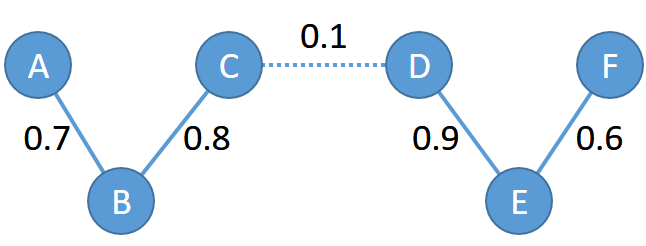
\includegraphics[width=7.5cm]{figures/谱聚类原理图.png}
\captionsetup{justification=centering}
\caption{谱聚类原理图 \\ Fig.\ref{谱聚类原理图} The Principle Diagram of the Spectral Clustering}\label{谱聚类原理图}
\end{figure}

在图\ref{谱聚类原理图}中,总共有$6$个节点,节点间连线上的数字表示两个节点间的相似度,如果现在要将这图分成两类,根据谱聚类的思想,应该去掉的边是用虚线表示的那一条边,这样就形成了两类节点。

由于本部分只使用到了非标准谱聚类算法,所以这里只介绍非标准谱聚类算法的执行步骤,谱聚类算法的步骤如下:

1. 假设输入数据的聚类数量为$k$,首先,定义数据之间相似度的度量标准,根据数据构造一个图,图的每一个节点对应一个数据点,将图中相邻的节点连接起来,数据之间的相似度用节点间边的权重来表示。把这个图用相似度矩阵的形式表示出来,记为$W$,相似度矩阵一般的计算公式为
$$
W_{ij}=\exp{(\frac{\|x_i-x_j\|^2}{2\sigma^2})}
$$

其中,$\sigma$为需要人工设定的参数,谱聚类算法的分类效果很大程度上取决于参数$\sigma$选取的合适与否;

2. 把相似度矩阵$W$中每一列的元素加起来得到$N$个数,把他们放到对角线上构成一个$N\times N$的对角矩阵,记为$D$,计算非标准化图的拉普拉斯矩阵$L=D-W$;

3. 求出$L$的前$k$个最小的特征值,以及特征值对应的特征向量$u_1,\cdots,u_k$;

4. 将这$k$个特征向量组成一个$N\times k$的矩阵$U$;

5. 将矩阵$U$的第$i$行作为行向量$(y_i)_{i=1,\cdots,n}$;

6. 对行向量$(y_i)_{i=1,\cdots,n}$使用$k$-means算法进行聚类,得到$k$个聚类$C_1,\cdots,C_k$[23]。

\begin{figure}[H]
    \centering
    \subfigure[聚类前原始数据]
    {
        \label{Fig.sub.1}
        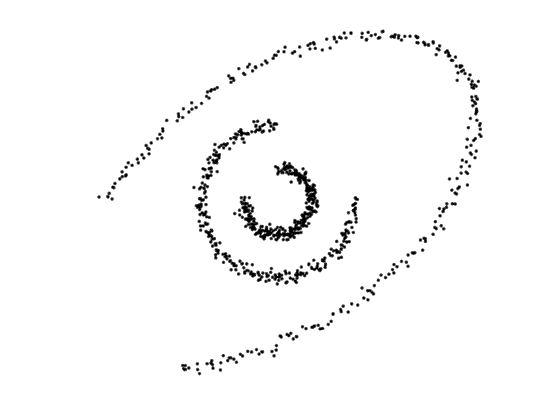
\includegraphics[width=3.8cm]{figures/聚类前原始数据.png}
    }
    \subfigure[谱聚类分类结果]
    {
        \label{Fig.sub.2}
        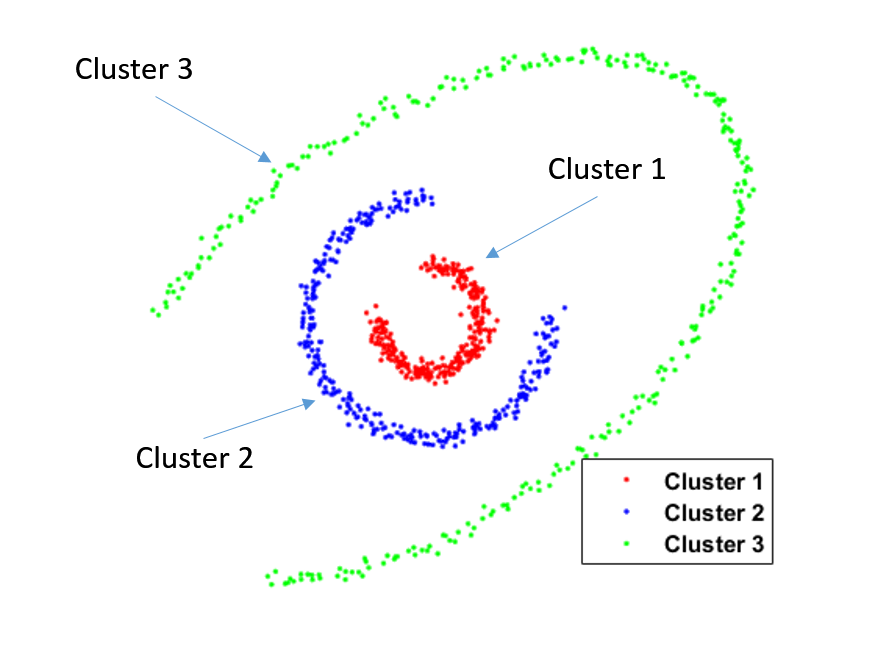
\includegraphics[width=3.8cm]{figures/谱聚类分类结果.png}
    }
    \captionsetup{justification=centering}
    \caption{谱聚类分类效果示意图 \\ Fig.\ref{谱聚类分类效果示意图} Spectral Clustering Classification Effect Diagram}
    \label{谱聚类分类效果示意图}
\end{figure}


谱聚类算法根据使用的相似度矩阵的不同,可以分成多种算法,其本质上是一类算法。

谱聚类和$k$-means算法比起来有很多优点:

(1) 谱聚类算法进行聚类的时候,只需要计算出数据之间的相似度矩阵即可,而$k$-means则要求数据必须是$N$维向量;

(2) 谱聚类算法对于一般的干扰误差数据不是很敏感;

(3) 运算复杂度比$k$-means小,在处理图像这种维度比较高的数据时,运行速度比$k$-means快;

(4) 能够避免得到局部最优解,从而获得全局最优解。


\subsection{区域邻接图简介}
区域邻接图(Region Adjacency Graph, RAG)定义为:$G=(V,E)$,其中$V_i$为节点,$E_{ij}$为边,相邻两节点间生成边,一般均为无向有权图,边的权值为两相邻节点之间的相似性度量,RAG表征区域间的空间相邻关系。

在图像分割中,首先使用预处理算法得到过分割的图像,其次,将过分割图像中的区域看作RAG中的节点,两相邻节点之间生成边,再根据相似度度量准则,生成过分割图像的RAG。


\begin{figure}[H]
    \centering
    \subfigure[初始分割结果]
    {
        \label{Fig.sub.1}
        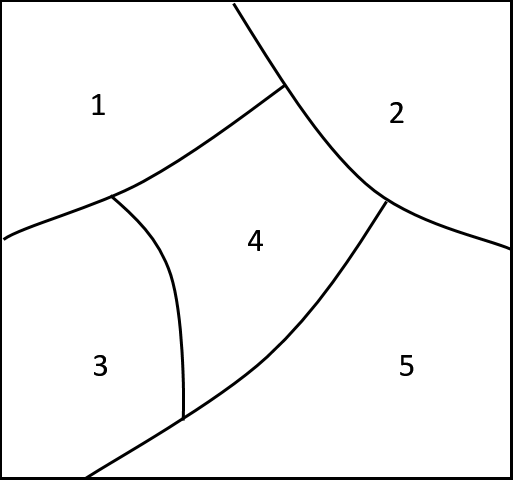
\includegraphics[width=3.8cm]{figures/初始分割结果.png}
    }
    \subfigure[对应的RAG]
    {
        \label{Fig.sub.2}
        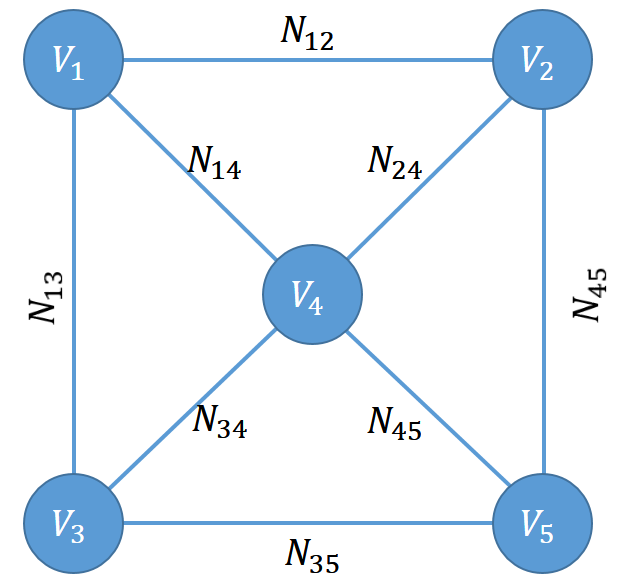
\includegraphics[width=3.8cm]{figures/对应的RAG.png}
    }
    \captionsetup{justification=centering}
    \caption{初始分割结果及其对应的RAG \\ Fig.\ref{初始分割结果及其对应的RAG} The Initial Segmentation Result and Its Corresponding RAG}
    \label{初始分割结果及其对应的RAG}
\end{figure}

使用RAG时,影响过分割图像合并结果的关键因素在于合并准则,主要有基于局部的合并准则和面向全局的合并准则两类。前者在局部范围内搜索满足合并条件的区域,并进行合并。后者从合并初始阶段开始,逐次合并全局最优的两个相邻区域,直到满足合并终止条件。面向全局的合并准则每次搜索全局最优的相邻区域进行合并,能及时针对每次合并产生的变化作出调整,精度较高,在合并准则确定的情况下,对于同一幅图像的合并过程相同,分割过程稳定性较好。合并准则中具体涵盖的特征多包括面积、均值、方差等初级视觉特征,而基于人体知觉的语义特征等高级特征较少应用于区域合并。

图\ref{RAG算法运算结果示意图}为RAG算法运算结果的示意图,图像中,黑色的边为SLIC算法分割出来的超像素块的边界,黄色的点为RAG中的图节点,绿色的边为RAG中图节点之间的边,不存在RAG边的地方表示图节点相似度较低,RAG算法将图节点之间的边擦除掉了。原始图像中,包括背景的底色共有5种颜色,经过RAG算法的处理,可以明显看出,不同颜色的超像素块之间的RAG边消失,相同颜色的超像素块之间的RAG边依旧存在。

\begin{figure}[H]
    \centering
    \subfigure[RAG原始图像]{
    \label{Fig.sub.1}
    
\includegraphics[width=3.8cm]{figures/RAG原始图像.jpg}}
    \subfigure[SLIC和RAG分割结果]{
    \label{Fig.sub.2}
    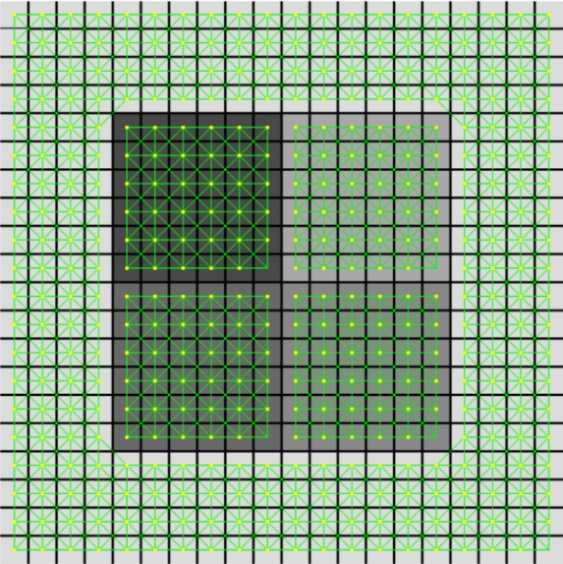
\includegraphics[width=3.8cm]{figures/SLIC算法和RAG算法分割结果.jpg}}
    \captionsetup{justification=centering}
    \caption{RAG算法运算结果示意图 \\ Fig.\ref{RAG算法运算结果示意图} RAG Algorithm Operation Result Diagram}
    \label{RAG算法运算结果示意图}
\end{figure}



\subsection{基于谱聚类和区域邻接图的最优分割算法}
基于谱聚类和区域邻接图的最优分割算法主要包括三个过程:SLIC算法进行图像过分割、谱聚类算法初次合并和区域邻接图进一步合并。下面依次介绍这三个过程。

(1) SLIC算法进行图像过分割

使用SLIC算法对输入原始图像进行过分割,在SLIC算法中,需要设定的参数有两个:超像素数量和紧密度参数。在本算法中,紧密度参数取值为常数$20$,超像素数量需要根据图像大小、景物大小、图像内容复杂度和算法应用场景进行设定,经过大量试验,对于Berkeley图像数据库(图像大小为$481\times321$)中的图像,兼顾算法运行时间,超像素数量设定为$500$即可。对于更大的图像,适当增加超像素数量能够提高算法分割质量。

(2) 谱聚类算法初步合并 

在使用 SLIC 算法对原始图像进行过分割生成超像素之后,首先进行超像素块的谱聚类过程。

对每一个超像素块,我们提取其$5$个特征构造相似度矩阵:包括$Lab$颜色空间超像素块的$l,a,b$颜色分量的均值,以及其等效位置$ x $坐标和$ y $坐标。

假设 SLIC 算法生成了$ N $个超像素块,则第$ i $个超像素块和第$ j $个超像素块间的距离将通过以下公式求得:
\[\begin{split}
D_{i,j}&=\sqrt{A_{i,j}+B_{i,j}} \\
A_{i,j}&=(l_i-l_j)^2+(a_i-a_j)^2+(b_i-b_j)^2 \\
B_{i,j}&=\frac{x_i-x_j}{SW}^2+\frac{y_i-y_j}{SW}^2
% D_{ij=√((l_i-l_j )^2+(a_i-a_j )^2+(b_i-b_j )^2+((x_i-x_j)/SW)^2+((y_i-y_j)/SW)^2 )
\end{split}\]

其中,$l,a,b$是超像素块在$Lab$颜色空间的颜色值,$x,y$是超像素块的等效位置。
$$
SW=\sqrt{((H\times W)/m)}
$$
$H$和$W$为图像的长度和宽度,$m$为一个常数,取值为$100$。

计算出距离矩阵$D$之后,对每一个超像素块,我们选择离它最近的$t$个超像素作为其邻居,则相似度矩阵$S$可以定义如下:
\begin{displaymath}
S_{i,j} = \left\{ \begin{array}{ll}

\exp{(\frac{-D^2_{i,j}}{2\sigma_i\sigma_j})}, & \textrm{超像素$i$和超像素$j$相邻}\\
0, & \textrm{其他}

\end{array} \right.
\end{displaymath}

其中,
$$
\sigma_i=\frac{1}{t}\sum_{k\in T}D_{i,k}
$$

超像素块$ k $属于超像素块$ i $的邻居超像素块的集合$T$。为了提高运行速度,将$t$取值为$5$。

得到相似度矩阵$S_{i,j}$之后,设定谱聚类算法的聚类数量,使用谱聚类算法进行聚类过程,实现超像素块的初步合并。

聚类数量的设定会影响谱聚类算法合并结果,如果聚类数量设定的不合理,会造成原始图像的欠分割,经过反复试验,针对,Berkeley图像数据库(图像大小为$481\times321$)和真实无人机航拍图像(图像大小为$1000\times1000$)而言,谱聚类数量设定为$30$时,谱聚类合并结果较为理想,当图像大小更大、内容较为复杂时,增加聚类数量能够得到更好的结果。

(3) 区域邻接图进一步合并

谱聚类算法对过分割图像的合并过程中,主要的合并依据为相似度矩阵$S$。在构造相似度矩阵$S$的过程中,超像素块之间的相似度主要通过公式进行计算,上式中,主要考虑了某一个超像素块在全局范围内与哪一个超像素块最相似,进而依据全局范围内的相似性进行聚类合并。RAG则将区域合并的重点放在衡量某一个超像素块与周围超像素块的相似性上。也就是说谱聚类算法的合并过程是一种面向全局的区域合并过程,而RAG的合并过程则是一种面向局部的区域合并过程,两种算法配合使用,能够兼顾全局和局部超像素块的相似性度量和合并。

在对谱聚类算法合并结果进行RAG区域合并的过程中,主要的参数为区域相似度阈值。当两个区域的相似度小于阈值时,合并这两个区域,反之不进行合并。区域相似度阈值$threshold$通过自适应的方式进行设定,以下对自适应方法进行介绍。

定义阈值$threshold$为变量$T$。同时,定义变量$MaxEdges$,其定义为在$Lab$颜色空间中,超像素块$k$与相邻超像素块集合$L$的最大颜色距离,$l\in L$时,颜色距离定义为:
$$
E_{k,l}=\sqrt{(l_i-l_j)^2+(a_i-a_j)^2+(b_i-b_j)^2}
$$

则$MaxEdges$定义为:
$$
MaxEdges=\max{(E_{k,l}),l\in L}
$$

$MaxEdges$求出来之后,可以求得$T$
$$
T=mean{(MaxEdges)}-\frac{std(MaxEdges)}{2}
$$

$mean(MaxEdges)$为$MaxEdges$的均值,$std(MaxEdges)$为$MaxEdges$ 的标准差。

为了避免阈值$T$过小影响合并过程,重新定义$T$如下:

\begin{displaymath}
T' = \left\{ \begin{array}{ll}

T, & \textrm{if $T>10$}\\
10, & \textrm{otherwise}

\end{array} \right.
\end{displaymath}



\section{实验结果}
\subsection{实验数据介绍}


本部分实验数据分为两部分,一部分为Berkeley图像数据库BSDS500,另一部分为真实无人机航拍图像。使用Berkeley图像数据库主要是为了对比基于单像素和基于超像素两种最优分割算法的分割结果,并且在Berkeley图像数据库中自然景物图像中,目标物体一般只有一个,便于定性评估最优分割算法。使用无人机航拍图像主要是为了评估算法在复杂场景中的表现。

\begin{figure}[H]
\centering
    \subfigure[BSDS12003]
    {
        \label{Fig.sub.1}
        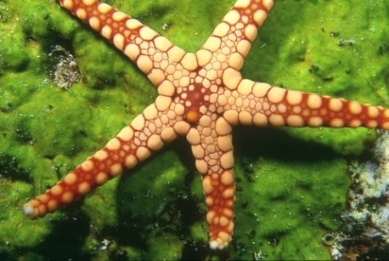
\includegraphics[width=2.4cm]{figures/BSDS12003.jpg}
    }
    \subfigure[BSDS118035]
    {
        \label{Fig.sub.1}
        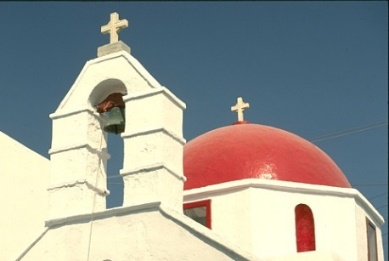
\includegraphics[width=2.4cm]{figures/BSDS118035.jpg}
    }
    \subfigure[BSDS8068]
    {
        \label{Fig.sub.1}
        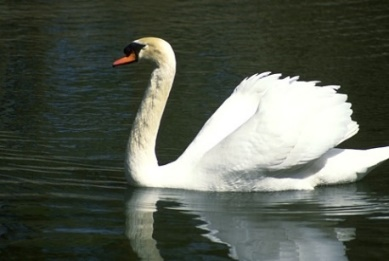
\includegraphics[width=2.4cm]{figures/BSDS8068.jpg}
    }
    \captionsetup{justification=centering}
    \caption{Berkeley 图像数据库 BSDS500 中的三张图像 \\ Fig.\ref{Berkeley图像数据库BSDS500中的三张图像} Three of the Berkeley Image Database BSDS500 Images}\label{Berkeley图像数据库BSDS500中的三张图像}
\end{figure}



\begin{figure}[H]
\centering
    \subfigure[航拍图像1]
    {
        \label{Fig.sub.1}
        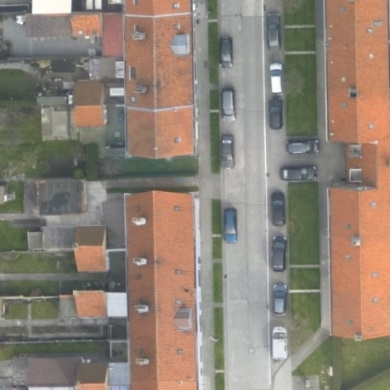
\includegraphics[width=2.4cm]{figures/无人机航拍图像1.jpg}
    }
    \subfigure[航拍图像2]
    {
        \label{Fig.sub.1}
        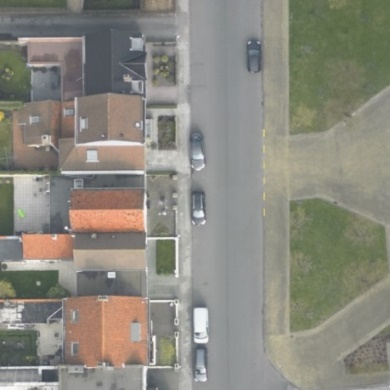
\includegraphics[width=2.4cm]{figures/无人机航拍图像2.jpg}
    }
    \subfigure[航拍图像3]
    {
        \label{Fig.sub.1}
        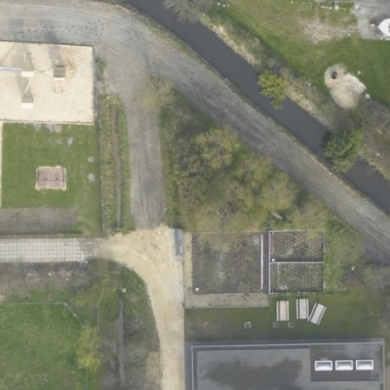
\includegraphics[width=2.4cm]{figures/无人机航拍图像3.jpg}
    }
    \captionsetup{justification=centering}
    \caption{三张无人机航拍图像 \\ Fig.\ref{三张无人机航拍图像} Three Unmanned Aerial Images}\label{三张无人机航拍图像}
\end{figure}





\subsection{基于单像素的最优分割算法实验结果}
本部分使用 Berkeley 图像数据库BSDS500进行实验。在SRM算法中,需要设定的参数为$Q$,$Q$ 的取值不同,所得分割效果不同。以下实验结果为$9$种$Q$值的SRM实验结果,从左到右从上到下依次为$Q={ 256,128,64,32,16,8,4,2,1}$。

\begin{figure}[H]
\centering
    \subfigure[SRM结果线图]
    {
        \label{Fig.sub.1}
        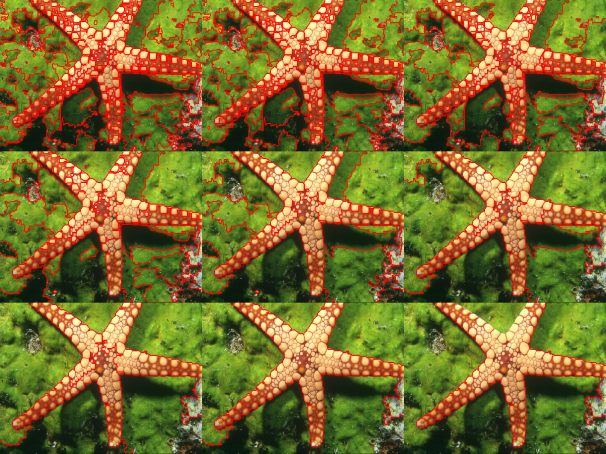
\includegraphics[width=3.5cm]{figures/图像BSDS12003的SRM结果线图.png}
    }
    \subfigure[SRM结果颜色图]
    {
        \label{Fig.sub.1}
        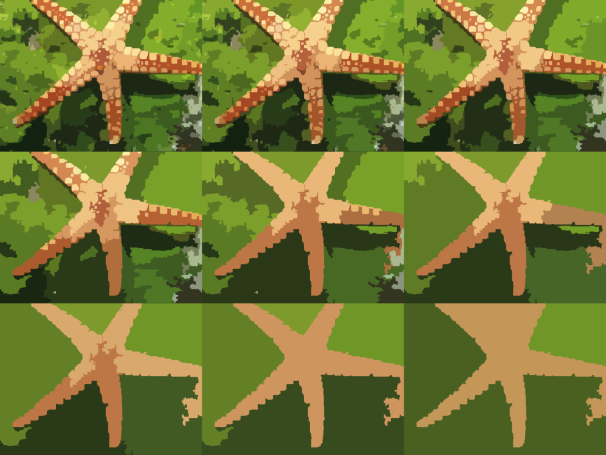
\includegraphics[width=3.5cm]{figures/图像BSDS12003的SRM结果颜色图.png}
    }
    \captionsetup{justification=centering}
    \caption{图像BSDS12003的SRM结果图 \\ Fig.\ref{SRM结果图1} Results Image BSDS12003 SRM are Illustrated}\label{SRM结果图1}
\end{figure}


\begin{figure}[H]
\centering
    \subfigure[SRM结果线图]
    {
        \label{Fig.sub.1}
        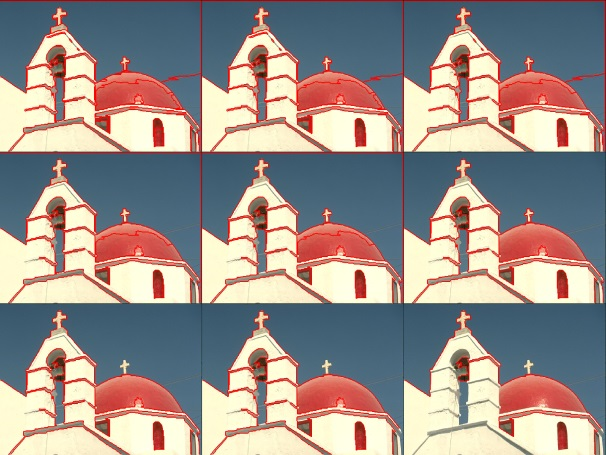
\includegraphics[width=3.5cm]{figures/图像BSDS118035的SRM结果线图.jpg}
    }
    \subfigure[SRM结果颜色图]
    {
        \label{Fig.sub.1}
        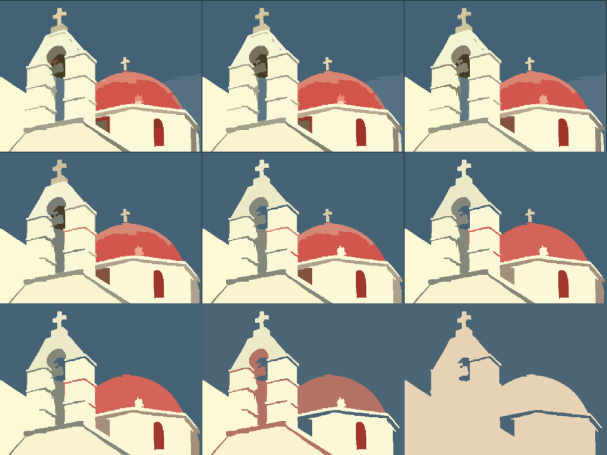
\includegraphics[width=3.5cm]{figures/图像BSDS118035的SRM结果颜色图.png}
    }
    \captionsetup{justification=centering}
    \caption{图像BSDS118035的SRM结果图 \\ Fig.\ref{SRM结果图2} Results Image BSDS118035 SRM are Illustrated}\label{SRM结果图2}
\end{figure}


\begin{figure}[H]
\centering
    \subfigure[SRM结果线图]
    {
        \label{Fig.sub.1}
        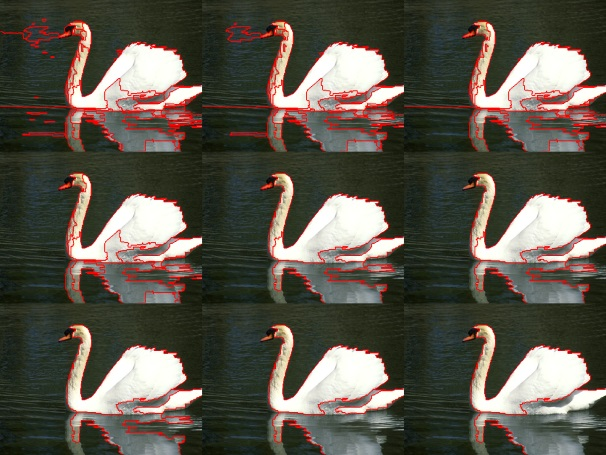
\includegraphics[width=3.5cm]{figures/图像BSDS8068的SRM结果线图.jpg}
    }
    \subfigure[SRM结果颜色图]
    {
        \label{Fig.sub.1}
        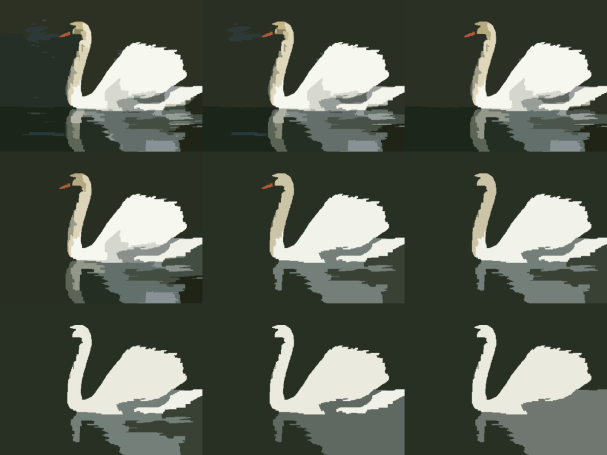
\includegraphics[width=3.5cm]{figures/图像BSDS8068的SRM结果颜色图.png}
    }
    \captionsetup{justification=centering}
    \caption{图像BSDS8068的SRM结果图 \\ Fig.\ref{SRM结果图3} Results Image BSDS8068 SRM are Illustrated}\label{SRM结果图3}
\end{figure}


\subsection{基于超像素表达的最优分割算法实验结果}

本部分实验使用基于超像素分割算法SLIC算法、聚类合并算法和区域邻接图RAG设计的面向目标提取的最优分割算法。

本部分实验的原始图像分为两部分:Berkeley图像数据库BSDS500和真实无人机航拍图像。针对上述两部分图像,调整必要参数,得到最优分割结果。由于谱聚类算法和RAG在本算法中的本质都是进行区域合并,所以本部分实验结果也分成两部分进行展示:包括谱聚类聚类区域合并结果和在谱聚类基础上的RAG区域合并结果。

\noindent{\textbf{(1) BSDS500数据库图像实验结果}}
\begin{figure}[H]
\centering
    \subfigure[谱聚类结果线图]
    {
        \label{Fig.sub.1}
        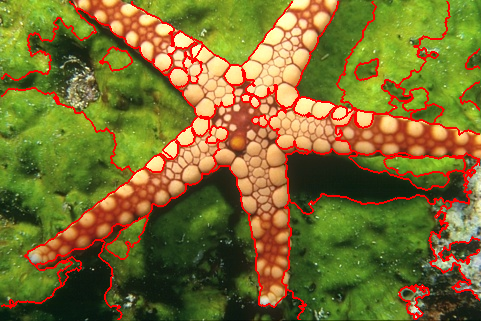
\includegraphics[width=3.5cm]{figures/图像BSDS12003的谱聚类结果线图.png}
    }
    \subfigure[谱聚类结果颜色图]
    {
        \label{Fig.sub.1}
        
\includegraphics[width=3.5cm]{figures/图像BSDS12003的谱聚类结果颜色图.png}
    }
    \subfigure[RAG结果线图]
    {
        \label{Fig.sub.1}
        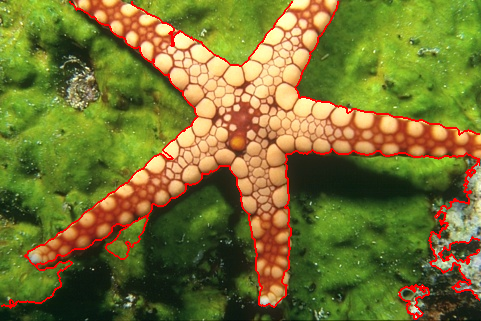
\includegraphics[width=3.5cm]{figures/图像BSDS12003的RAG结果线图.png}
    }
    \subfigure[RAG结果颜色图]
    {
        \label{Fig.sub.1}
        
\includegraphics[width=3.5cm]{figures/图像BSDS12003的RAG结果颜色图.png}
    }
    \captionsetup{justification=centering}
    \caption{图像BSDS12003的最优分割结果 \\ Fig.\ref{最优分割结果1} The image of BSDS12003 optimal segmentation result}\label{最优分割结果1}
\end{figure}

\begin{figure}[H]
\centering
    \subfigure[谱聚类结果线图]
    {
        \label{Fig.sub.1}
        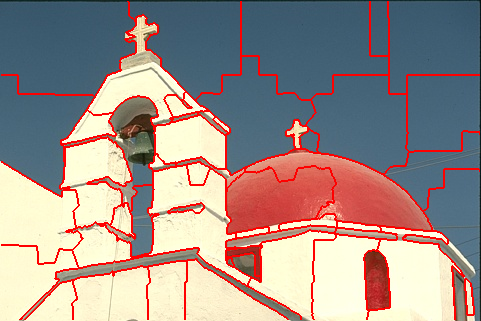
\includegraphics[width=3.5cm]{figures/图像BSDS118035的谱聚类结果线图.png}
    }
    \subfigure[谱聚类结果颜色图]
    {
        \label{Fig.sub.1}
        
\includegraphics[width=3.5cm]{figures/图像BSDS118035的谱聚类结果颜色图.png}
    }
    \subfigure[RAG结果线图]
    {
        \label{Fig.sub.1}
        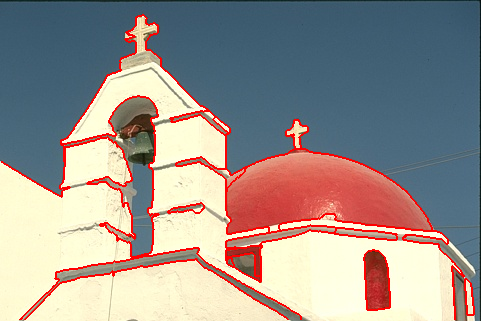
\includegraphics[width=3.5cm]{figures/图像BSDS118035的RAG结果线图.png}
    }
    \subfigure[RAG结果颜色图]
    {
        \label{Fig.sub.1}
        
\includegraphics[width=3.5cm]{figures/图像BSDS118035的RAG结果颜色图.png}
    }
    \captionsetup{justification=centering}
    \caption{图像BSDS118035的最优分割结果 \\ Fig.\ref{最优分割结果2} The image of BSDS118035 optimal segmentation result}\label{最优分割结果2}
\end{figure}


\begin{figure}[H]
\centering
    \subfigure[谱聚类结果线图]
    {
        \label{Fig.sub.1}
        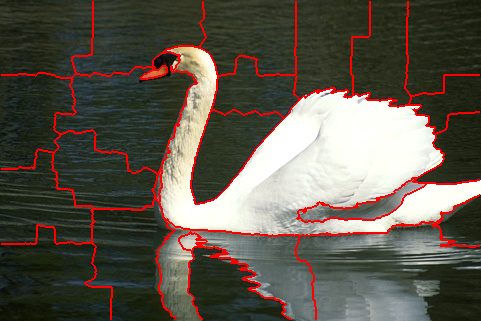
\includegraphics[width=3.5cm]{figures/图像BSDS8068的谱聚类结果线图.png}
    }
    \subfigure[谱聚类结果颜色图]
    {
        \label{Fig.sub.1}
        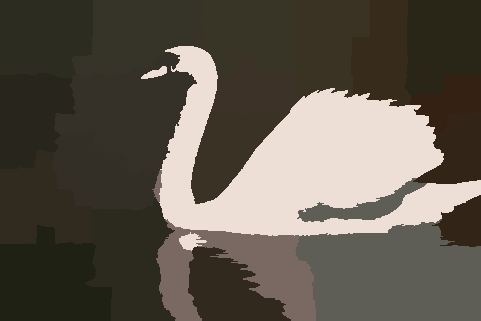
\includegraphics[width=3.5cm]{figures/图像BSDS8068的谱聚类结果颜色图.png}
    }
    \subfigure[RAG结果线图]
    {
        \label{Fig.sub.1}
        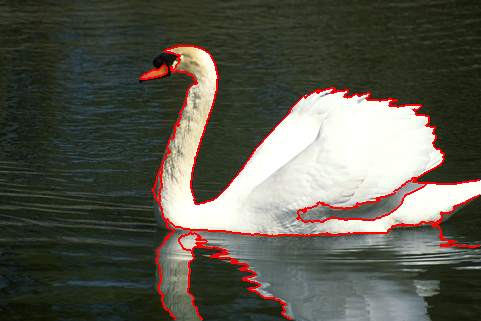
\includegraphics[width=3.5cm]{figures/图像BSDS8068的RAG结果线图.png}
    }
    \subfigure[RAG结果颜色图]
    {
        \label{Fig.sub.1}
        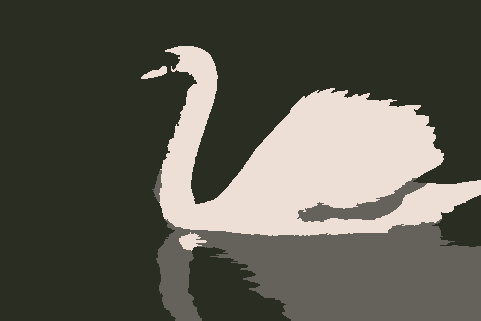
\includegraphics[width=3.5cm]{figures/图像BSDS8068的RAG结果颜色图.png}
    }
    \captionsetup{justification=centering}
    \caption{图像BSDS8068的最优分割结果 \\ Fig.\ref{最优分割结果3} The image of BSDS8068 optimal segmentation result}\label{最优分割结果3}
\end{figure}

\noindent{\textbf{(2) 无人机航拍图像实验结果}}


\begin{figure}[H]
\centering
    \subfigure[谱聚类结果线图]
    {
        \label{Fig.sub.1}
        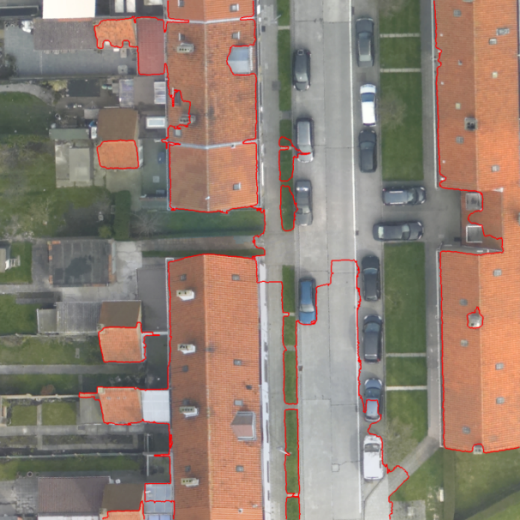
\includegraphics[width=3.2cm]{figures/无人机航拍图像1RAG结果线图.png}
    }
    \subfigure[谱聚类结果颜色图]
    {
        \label{Fig.sub.1}
        
\includegraphics[width=3.2cm]{figures/无人机航拍图像1RAG结果颜色图.png}
    }
    \subfigure[RAG结果线图]
    {
        \label{Fig.sub.1}
        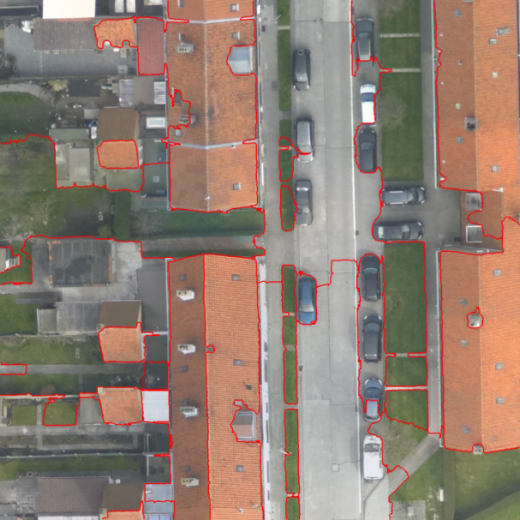
\includegraphics[width=3.2cm]{figures/无人机航拍图像1谱聚类结果线图.png}
    }
    \subfigure[RAG结果颜色图]
    {
        \label{Fig.sub.1}
        
\includegraphics[width=3.2cm]{figures/无人机航拍图像1谱聚类结果颜色图.png}
    }
    \captionsetup{justification=centering}
    \caption{无人机航拍图像1的最优分割结果 \\ Fig.\ref{无人机最优分割结果1} 1 the optimal segmentation result unmanned aerial images}\label{无人机最优分割结果1}
\end{figure}


\begin{figure}[H]
\centering
    \subfigure[谱聚类结果线图]
    {
        \label{Fig.sub.1}
        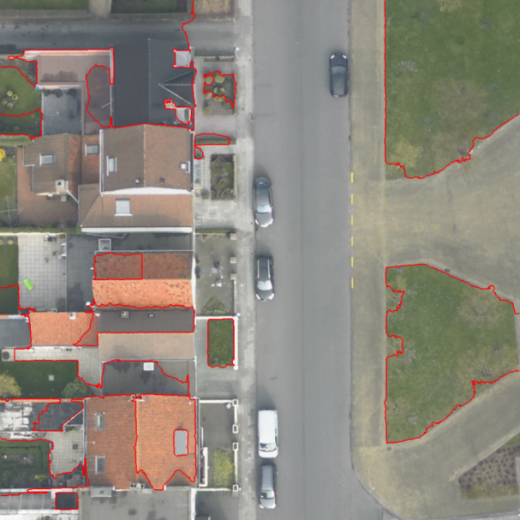
\includegraphics[width=3.2cm]{figures/无人机航拍图像2RAG结果线图.png}
    }
    \subfigure[谱聚类结果颜色图]
    {
        \label{Fig.sub.1}
        
\includegraphics[width=3.2cm]{figures/无人机航拍图像2RAG结果颜色图.png}
    }
    \subfigure[RAG结果线图]
    {
        \label{Fig.sub.1}
        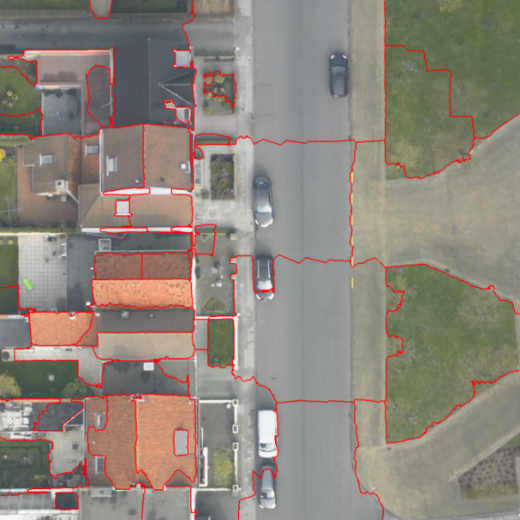
\includegraphics[width=3.2cm]{figures/无人机航拍图像2谱聚类结果线图.png}
    }
    \subfigure[RAG结果颜色图]
    {
        \label{Fig.sub.1}
        
\includegraphics[width=3.2cm]{figures/无人机航拍图像2谱聚类结果颜色图.png}
    }
    \captionsetup{justification=centering}
    \caption{无人机航拍图像2的最优分割结果\\ Fig.\ref{无人机最优分割结果2} 2 the optimal segmentation result unmanned aerial images}\label{无人机最优分割结果2}
\end{figure}


\begin{figure}[H]
\centering
    \subfigure[谱聚类结果线图]
    {
        \label{Fig.sub.1}
        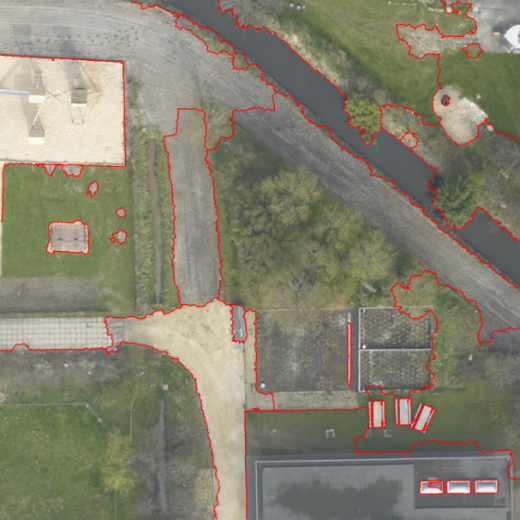
\includegraphics[width=3.2cm]{figures/无人机航拍图像3RAG结果线图.png}
    }
    \subfigure[谱聚类结果颜色图]
    {
        \label{Fig.sub.1}
        
\includegraphics[width=3.2cm]{figures/无人机航拍图像3RAG结果颜色图.png}
    }
    \subfigure[RAG结果线图]
    {
        \label{Fig.sub.1}
        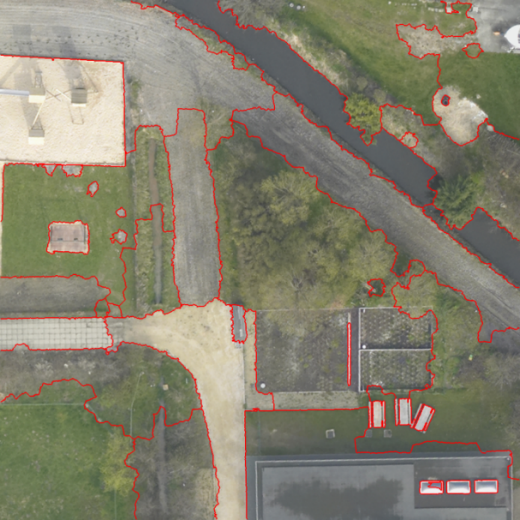
\includegraphics[width=3.2cm]{figures/无人机航拍图像3谱聚类结果线图.png}
    }
    \subfigure[RAG结果颜色图]
    {
        \label{Fig.sub.1}
        
\includegraphics[width=3.2cm]{figures/无人机航拍图像3谱聚类结果颜色图.png}
    }
    \captionsetup{justification=centering}
    \caption{无人机航拍图像3的最优分割结果\\ Fig.\ref{无人机最优分割结果3} 3 the optimal segmentation result unmanned aerial images}\label{无人机最优分割结果3}
\end{figure}



\subsection{实验结果分析}

由图\ref{SRM结果图1}和\ref{SRM结果图2}可以清楚的看出,$Q$取值不同,分割结果不同,$Q$值越小,分割结果中聚类数量越少,当$Q$取值合理的时候,能将前景目标与背景分离出来。

本部分实验使用两部分数据进行实验,一部分是Berkeley图像数据库,另一部分是真实的无人机航拍图像。
由图\ref{最优分割结果1}、\ref{最优分割结果2}和\ref{最优分割结果3}可以清楚的看出,经过谱聚类和RAG两次区域合并,能将大部分的超像素块正确进行合并,并将前景目标和背景进行分离。但是,同时由图\ref{无人机最优分割结果1}、\ref{无人机最优分割结果2}和\ref{无人机最优分割结果3}能够看出,基于超像素的最优分割算法在场景较为复杂的时候分割效果不够理想,许多超像素块被错误合并。


\section{结语}
在使用 SLIC 算法对图像进行超像素表达的基础上,将谱聚类算法和区域邻接图相结合,完成了基于超像素表达的面向目标提取最优分割算法的设计。并对本部分算法在Berkeley图像数据库BSDS500和真实无人机航拍图像上的表现进行了定性评估。通过实验,本设计在BSDS500这种前景目标较为简单的自然图像上表现较好,但是在真实无人机航拍图像上表现不是很好,有很大的提升空间。

%%%%%%%%%%%%%%%%%%%%%%%%%%%%%%%%%%%%%%%%%%%%%%%%%%%%%%%%%%%%%%%%
%  参考文献
%%%%%%%%%%%%%%%%%%%%%%%%%%%%%%%%%%%%%%%%%%%%%%%%%%%%%%%%%%%%%%%%
\small

\begin{thebibliography}{99}
    \setlength{\parskip}{0pt}  %段落之间的竖直距离

    \bibitem{超像素1} 王春瑶, 陈俊周, 李炜. 超像素分割算法研究综述[J]. 计算机应用研究, 2014(01 vo v.31; No.267): 6-12.

    \bibitem{超像素2} 宋熙煜, 周利莉, 李中国等. 图像分割中的超像素方法研究综述[J]. 中国图象图形学报, 2015(05 vo v.20; No.229): 599-608.

    \bibitem{区域合并算法} Nock R, Nielsen F. Statistical region merging[J]. IEEE Transactions on Pattern Analysis and Machine Intelligence, 2004, 26(11): 1452–1458.

    \bibitem{谱聚类算法2} Ng A Y, Jordan M I, Weiss Y. On Spectral Clustering: Analysis and an algorithm[A]. ADVANCES IN NEURAL INFORMATION PROCESSING SYSTEMS[C]. MIT Press, 2001: 849-856.

    \bibitem{谱聚类算法3} Luxburg U von. A tutorial on spectral clustering[J]. Statistics and Computing, 2007, 17(4): 395-416.

    \bibitem{谱聚类算法4} Zelnik-manor L, Perona P. Self-Tuning Spectral Clustering[A]. see: L.K. Saul, Y. Weiss, L. Bottou. Advances in Neural Information Processing Systems 17[M]. MIT Press, 2005: 1601-1608.

    \bibitem{谱聚类算法5} 林泽桢. 聚类分析中基于密度算法的研究与改进[D]. 复旦大学, 2013.

    \bibitem{谱聚类算法6} Tremeau A, Colantoni P. Regions adjacency graph applied to color image segmentation[J]. IEEE Transactions on Image Processing, 2000, 9(4): 735-744.

    \bibitem{谱聚类算法7} 肖鹏峰, 冯学智. 高分辨率遥感图像分割与信息提取[M]. 北京: 科学出版社, 2012.

   \bibitem{谱聚类算法8} 门学敏. 基于图论的超像素分割及其合并算法[D]. 燕山大学, 2014.


\end{thebibliography}

%%%%%%%%%%%%%%%%%%%%%%%%%%%%%%%%%%%%%%%%%%%%%%%%%%%%%%%%%%%%%%%%
% 作者简历,段落插入图片用picins宏包和\parpic命令
%%%%%%%%%%%%%%%%%%%%%%%%%%%%%%%%%%%%%%%%%%%%%%%%%%%%%%%%%%%%%%%%
% \normalsize


%%%%%%%%%%%%%%%%%%%%%%%%%%%%%%%%%%%%%%%%%%%%%%%%%%%%%%%%%%%%%%%%
%  分栏结束
%%%%%%%%%%%%%%%%%%%%%%%%%%%%%%%%%%%%%%%%%%%%%%%%%%%%%%%%%%%%%%%%
\end{multicols}

%%%%%%%%%%%%%%%%%%%%%%%%%%%%%%%%%%%%%%%%%%%%%%%%%%%%%%%%%%%%%%%%
%  英文摘要
%%%%%%%%%%%%%%%%%%%%%%%%%%%%%%%%%%%%%%%%%%%%%%%%%%%%%%%%%%%%%%%%
\vspace{.1cm}
\begin{center}


\parbox{\textwidth}{

\begin{center}
{\zihao{-2} {\textbf{An Optimal Image Segmentation Algorithm for Object Extraction on the Basis of Superpixel Algorithm}}}\\
\vspace{0.1cm}
\end{center}


\begin{center}
\zihao{5}\textit{WANG Jinwang}\\
\zihao{6}{School of Electronic and Information,Wuhan University, Wuhan 430079, China}\\
\end{center}

{\zihao{5}{\textbf{Abstract:~}In the paper, we have studied an optimal image segmentation algorithm for object extraction on the basis of superpixel algorithm. Using SLIC to generate superpixel on the UAV aerial images, afterwares, on the basis of superpixels, using spectral clustering and RAG(Region Adjacency Graph) methods to merge superpixels. According to the results, we can get the optimal image segmentation. In addition, we use BSDS500, a Berkeley image database and UAV aerial images to condact experiments over the optimal image segmentation algorithm for object extraction. According to the result, the algorithm turns out to be effecitive.\\
\textbf{Key Words:~}UAV; aerial image; superpixel; segmentation}}
}
\end{center}

\end{document}